\documentclass[9pt]{beamer}

\usecolortheme[RGB={55,110,144}]{structure} % prima c'era questo bluetto: 20,104,204  % blu elettrico: 20,10,244

\usepackage{bbm,color,xcolor}
\usepackage[utf8]{inputenc}

\usepackage{fontenc,fancyvrb}

\usepackage{amsmath}
\usepackage{mathtools}
\usepackage{amssymb}
\usepackage{amsfonts}
\usepackage{graphicx}
\usepackage{mathrsfs}
\usepackage{pgfplots}

\definecolor{mycolor}{rgb}{0.28,0.69,0.7}
\definecolor{mycolor1}{rgb}{0.7,0.75,0.71}
\definecolor{mycolor2}{rgb}{0.58,1,1}

\usepackage{pifont}% http://ctan.org/pkg/pifont
\newcommand{\cmark}{\ding{51}}%
\newcommand{\xmark}{\ding{55}}%

\usepackage{amsmath,amssymb,amsthm,amscd,latexsym,tcolorbox,array}
\usepackage{amsfonts,mathrsfs,nomencl,hyperref,threeparttable,textcomp}
\usepackage[english]{babel}
\usepackage{graphicx,tabularx,tikz,setspace,subfigure,epigraph,lscape,color,booktabs,multirow}
\usepackage{fancybox}
\usetikzlibrary{plotmarks}
\usetikzlibrary{matrix}
\usetikzlibrary{positioning}
\usetikzlibrary{mindmap,backgrounds}

%% strange style
\usepackage{times}
%\usepackage{mathptmx}
%\usepackage[scaled=.90]{helvet}
%\usepackage{courier}

\usepackage[labelformat=empty,labelsep=none]{caption}
%\renewcommand{\tablename}{}

%\def\softO{\ensuremath{{\mathcal{O}}{\,\tilde{ }\,}}}

\addtobeamertemplate{footline}{\hfill\insertframenumber/\inserttotalframenumber}

\usepackage{color,xcolor,colortbl}

\definecolor{mycolor}{rgb}{0.28,0.69,0.7}
\definecolor{mycolor1}{rgb}{0.7,0.75,0.71}
\definecolor{mycolor2}{rgb}{0.58,1,1}

%\normalfont

\renewcommand{\familydefault}{\rmdefault}

\newcommand{\red}[1]{{\bf \color{red} #1}}

\newcommand{\calD}{\mathcal{D}}
\newcommand{\calZ}{\mathcal{Z}}
\newcommand{\minrank}{{r}(A)}

\newcommand{\rrY}{{\color{red} \bf Y}}

\newcommand{\bc}{\begin{center}}
\newcommand{\ec}{\end{center}}
\newcommand{\cit}{\color{olive}\bf}


\setbeamercolor{upcol}{fg=black,bg=green}      %\setbeamercolor{upcol}{fg=black,bg=orange} prima c'era questo
\setbeamercolor{lowcol}{fg=black,bg=green!40}  %\setbeamercolor{lowcol}{fg=black,bg=orange!40}

\setbeamertemplate{navigation symbols}{}

\theoremstyle{definition}
\newtheorem{prob}{Problem}[section]

\theoremstyle{definition}
\newtheorem{prop}{Proposition}[section]

\theoremstyle{definition}
\newtheorem{teo}{Theorem}[section]

\theoremstyle{definition}
\newtheorem{defin}{Definition}[section]

\theoremstyle{definition}
\newtheorem{coroll}{Corollary}[section]

\theoremstyle{definition}
\newtheorem{oss}{Remark}[section]

\title[]{\bf Title \smallskip \smallskip \smallskip}
\author{{\bf Tristan Vaccon} \\ \vspace{0.1cm} Université de Limoges}
\date{Tropical seminar \\ CMAP, École Polytechnique \\[.5cm] April 9, 2026}


%\usetheme{default}

% MACROS

%% Fields - Rings
\def\QQ{{\mathbbmss{Q}}} % rational numbers
\def\RR{{\mathbbmss{R}}} % real numbers
\def\CC{{\mathbbmss{C}}} % complex numbers
\def\ZZ{{\mathbbmss{Z}}} % integer numbers
\def\NN{{\mathbbmss{N}}} % natural numbers
\def\sym{{\mathbbmss{S}}} % symmetric matrices

\def\bigO{{\mathcal{O}}}

%% Polynomial families
\def\f{{\mathbf{f}}}
\def\g{{\mathbf{g}}}
\def\h{{\mathbf{h}}}
\def\q{{\mathbf{q}}}

%% For the section FERMETURE.TEX + NOETHER.TEX + BOUNDARY.TEX
\def\fermF{{\mathcal{F}}} % families F_i of varieties of dimension <= i
\def\fermD{{D}} % the equidimensional variety of all section about the properness of projections
\def\fermS{{\mathcal{S}}} % subvarieties of the singular locus of \fermD
\def\fermW{{\mathcal{W}}} % polar varieties of \fermD
\def\fermI{{\mathcal{I}}} % families of ideals
\def\fermT{{\mathcal{T}}} % a generic variety in F_i
\def\fermL{{\mathcal{L}}} % a set in the proof of boundary.tex
\def\fermU{{\mathfrak{A}}} % the parameters for the matrix \bfM in the proof of noether position
\def\fermP{{\mathcal{P}}} % a prime ideal
\def\fermQ{{\mathcal{Q}}} % a prime ideal
\def\sing{{\sf Sing}}
\def\crit{{\sf Crit}}
\def\reg{{\sf Reg}}
\def\scC{{\mathscr{C}}}
\def\scS{{\mathscr{S}}}
\def\sfP{{\mathsf{P}}}
\def\sfQ{{\mathsf{Q}}}
\def\spec{{\mathscr{S}}}
\def\poly{{\mathscr{P}}}

\def\Ideal{{\mathsf{Ideal}}}

%% Properties
\def\sfG{{\mathsf{G}}} % property G
\def\sfH{{\mathsf{H}}} % property H

%% Matrices
\def\sfA{{\mathsf{A}}} % the linear matrix
\def\GL{{\mathrm{GL}}} % the general linear group
\def\bfM{{\mathsf{M}}} % the matrix of change of variables
\def\rank{{\ensuremath{\mathsf{rank}}}} % rank function
\def\jac{{\ensuremath{\mathsf{jac}}}} % jacobian matrix
\def\minors{{\ensuremath{\mathsf{Minors}}}} % set of minors
\def\subm{{\ensuremath{\mathsf{SubMatrix}}}} % set of minors

%% Variables
\def\X{{X}} % variables of the space of the determinant
\def\Y{{Y}} % variables of the space of the incidence variety (kernel variables)
\def\Z{{Z}} % variables of the space of critical points (Lagrange multipliers)
\def\M{{M}}
\def\V{{V}}

%% Points
\def\x{{x}} % a generic first point
\def\y{{y}} % a generic second point
\def\z{{z}} % a generic third point
\def\v{{v}} % a generic third point
\def\fiber{{\alpha}} % a generic third point

%% Parameters
\def\fraka{{\mathfrak{a}}}
%\def\frakb{{\mathfrak{b}}}
%\def\frakc{{\mathfrak{c}}}
\def\fraku{{\mathfrak{u}}}
%\def\frakv{{\mathfrak{v}}}
\def\frakm{{\mathfrak{m}}}
\def\frakA{{\mathfrak{A}}}
%\def\frakB{{\mathfrak{B}}}
%\def\frakC{{\mathfrak{C}}}

\newcommand{\calV}{\mathcal{V}}

\def\Id{{\mathbb{I}}}

%% Algebraic sets
\def\setD{{\mathcal{D}}}
\def\setV{{\mathcal{V}}}
\def\setW{{\mathcal{W}}}
\def\spec{{\mathscr{S}}}

%% Zariski-open sets
\def\zarA{{\mathscr{A}}}
\def\zarfiber{{\mathscr{I}}}
\def\zarU{{\mathscr{U}}}
\def\zarV{{\mathscr{V}}}
\def\zarM{{\mathscr{M}}}
\def\zarU{{\mathscr{U}}}
\def\zarO{{\mathscr{O}}}

\def\softO{\ensuremath{{\mathcal{O}}{\,\tilde{ }\,}}}

\newcommand{\bX}{{x}}
\newcommand{\rY}{{y}}
\newcommand{\gZ}{{z}}

%% Messages
\def\mymid{{\,\,:\,\,}}
\definecolor{mycolor}{rgb}{0.28,0.69,0.7}
\definecolor{mycolor1}{rgb}{0.7,0.75,0.71}
\definecolor{mycolor2}{rgb}{0.58,1,1}
\def\fall{\forall\,}
\def\MM{{\mathbb{M}}}
\def\SS{{\mathbb{S}}}
\def\sing{{\rm sing}\,}
\def\crit{{\rm crit}\,}
\def\reg{{\rm reg}\,}
\def\minors{{\rm minors}\,}
\def\spec{\mathscr{S}}
\def\cc{\mathcal{C}}

\usetikzlibrary{positioning}
\usetikzlibrary{fit}
\usetikzlibrary{backgrounds}
\usetikzlibrary{calc}
\usetikzlibrary{shapes}

\tikzset{box1/.style={draw=black, thick, rectangle,rounded corners, minimum height=2cm, minimum width=2cm}}

\setbeamerfont{page number in head/foot}{size=\large}
\setbeamertemplate{footline}[frame number]
\setbeamercolor{page number in head/foot}{fg=black}

\begin{document}

%%%%%%%%%%%%%%%%%%%%%%%%%%%%%%%%%%%%%%%%%%%%%%%%%%%%%%%%%%%%%%%%%%%%%%%%%%%%%
\begin{frame}
  \maketitle
\end{frame}

%%%%%%%%%%%%%%%%%%%%%%%%%%%%%%%%%%%%%%%%%%%%%%%%%%%%%%%%%%%%%%%%%%%%%%%%%%%%%
\begin{frame}
\frametitle{\vspace{-0.5cm}\bc \bf Polyhedra and Spectrahedra over $\RR$ \ec}

\vspace{-0.5cm}
For $\ell_1,\ldots,\ell_m \in \RR[x]{\leq 1}$ real affine $n$-variate functions:

\begin{tcolorbox}[colback=green!5,colframe=blue!40!black]
  \bc Polyhedron: {\color{red} $\poly = \{x \in \RR^n \mymid \ell_i(x) \geq 0, i=1,\ldots,m\}$} \ec
\end{tcolorbox}

\pause
\vspace{0.2cm}

For $A_0,A_1,\ldots,A_n \in \sym^{m}$ real symmetric matrices

\begin{tcolorbox}[colback=green!18,colframe=blue!40!black]
  \bc Spectrahedron: {\color{red} $\spec = \{x \in \RR^n \mymid A(x)=A_0+x_1A_1+\cdots+x_nA_n \succeq 0\}$} \ec
  \vspace{-0.6cm}
  \hbox{}\hfill {\color{blue}\footnotesize ``$\succeq 0$'' = positive semi-definite = its eigenvalues are $\geq 0$.
    $A(x) \succeq 0$ is {\bf called} a {\bf LMI}.}
  \vspace{-0.2cm}
\end{tcolorbox}

\pause
\vspace{0.2cm}

{\bf\color{blue} Fact:}
Polyhedra are Spectrahedra, since $x \in \poly \Leftrightarrow A(x) \coloneqq \text{diag}(\ell_1,\ldots,\ell_m) \succeq 0$.

\pause
\vspace{0.2cm}

{\bf\color{blue} Fact:} Polyhedra resp. Spectrahedra are {\bf convex} as affine pre-images of resp.
\begin{equation*}
  \begin{aligned}
    \text{(nonnegative orthants)} \,\,\,\, \RR^m_+ &= \{y \in \RR^m : y_i \geq 0, i=1,\ldots,m\} \\
    \text{(positive semidefinite cones)} \,\,\,\, \sym^m_+ &= \{X \in \sym_m : X \succeq 0\}.   
  \end{aligned}
\end{equation*}

\pause
\vspace{0.2cm}

{\bf\color{blue} Fact:}
They are {\bf basic semi-algebraic} sets:
$$\det(A(x)+t I_m) = f_{m}(x)+f_{m-1}(x)t+\cdots+f_{1}(x)t^{m-1}+t^m$$
then $\spec=\{x \in \RR^n \mymid f_i(x) \geq 0, i=1,\ldots,m\}$.

\end{frame}


%%%%%%%%%%%%%%%%%%%%%%%%%%%%%%%%%%%%%%%%%%%%%%%%%%%%%%%%%%%%%%%%%%%%%%%%%%%%%
\begin{frame}
\frametitle{\vspace{-0.5cm} \bc \bf Polyhedra and Spectrahedra over $\RR$\ec}
  \begin{figure}[H]
    \centering
    \vspace{-0.6cm}
    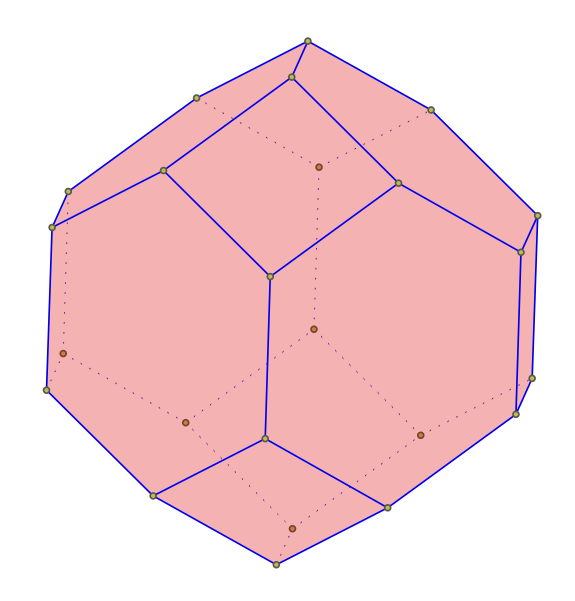
\includegraphics[width=.3\linewidth]{IMAGES/polytope}
    \hspace{1.5cm}
    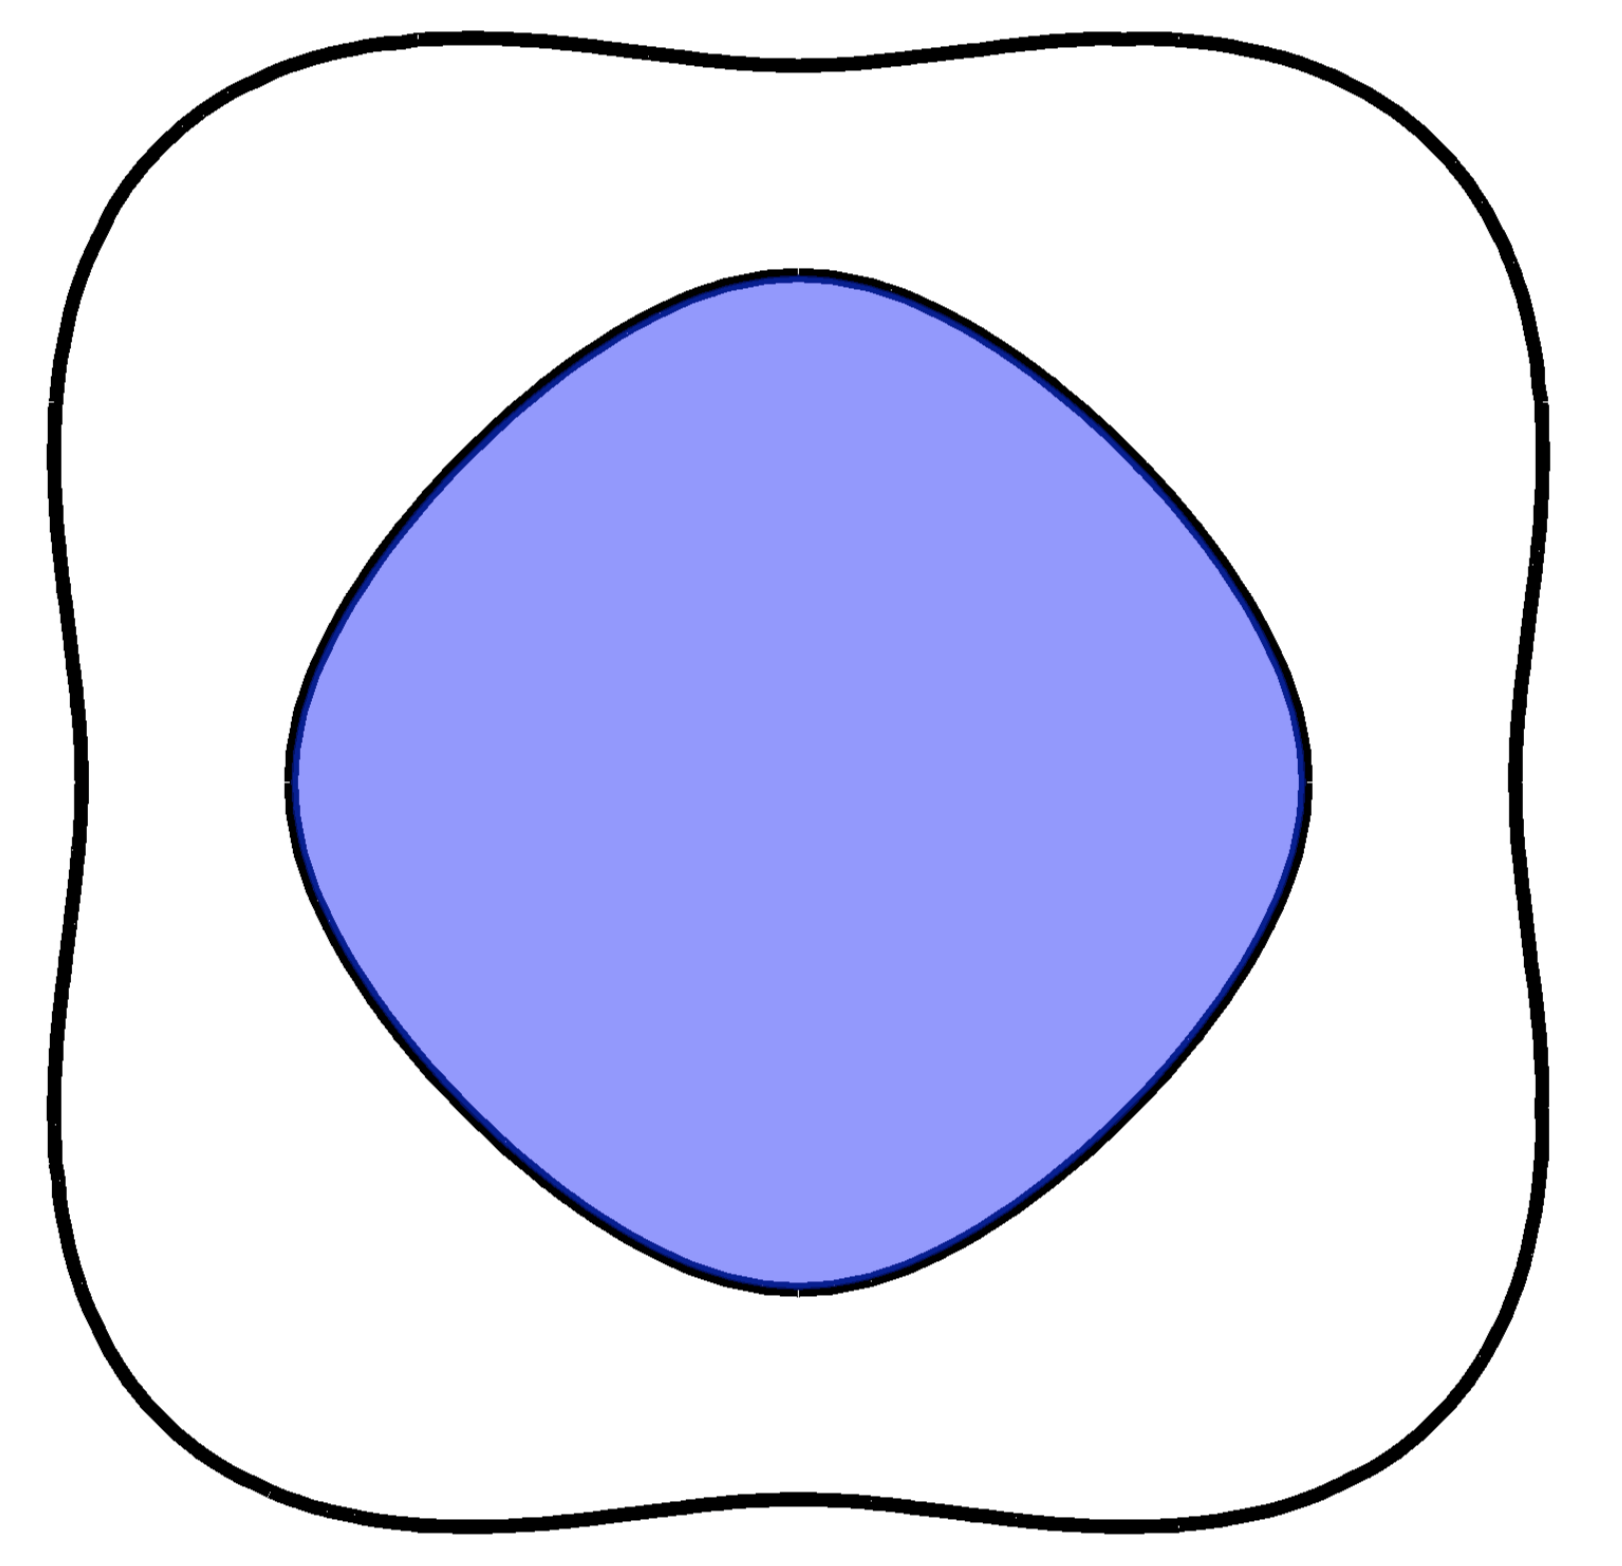
\includegraphics[width=.3\linewidth]{IMAGES/hypcone} \\
    \vspace{0.1cm}
    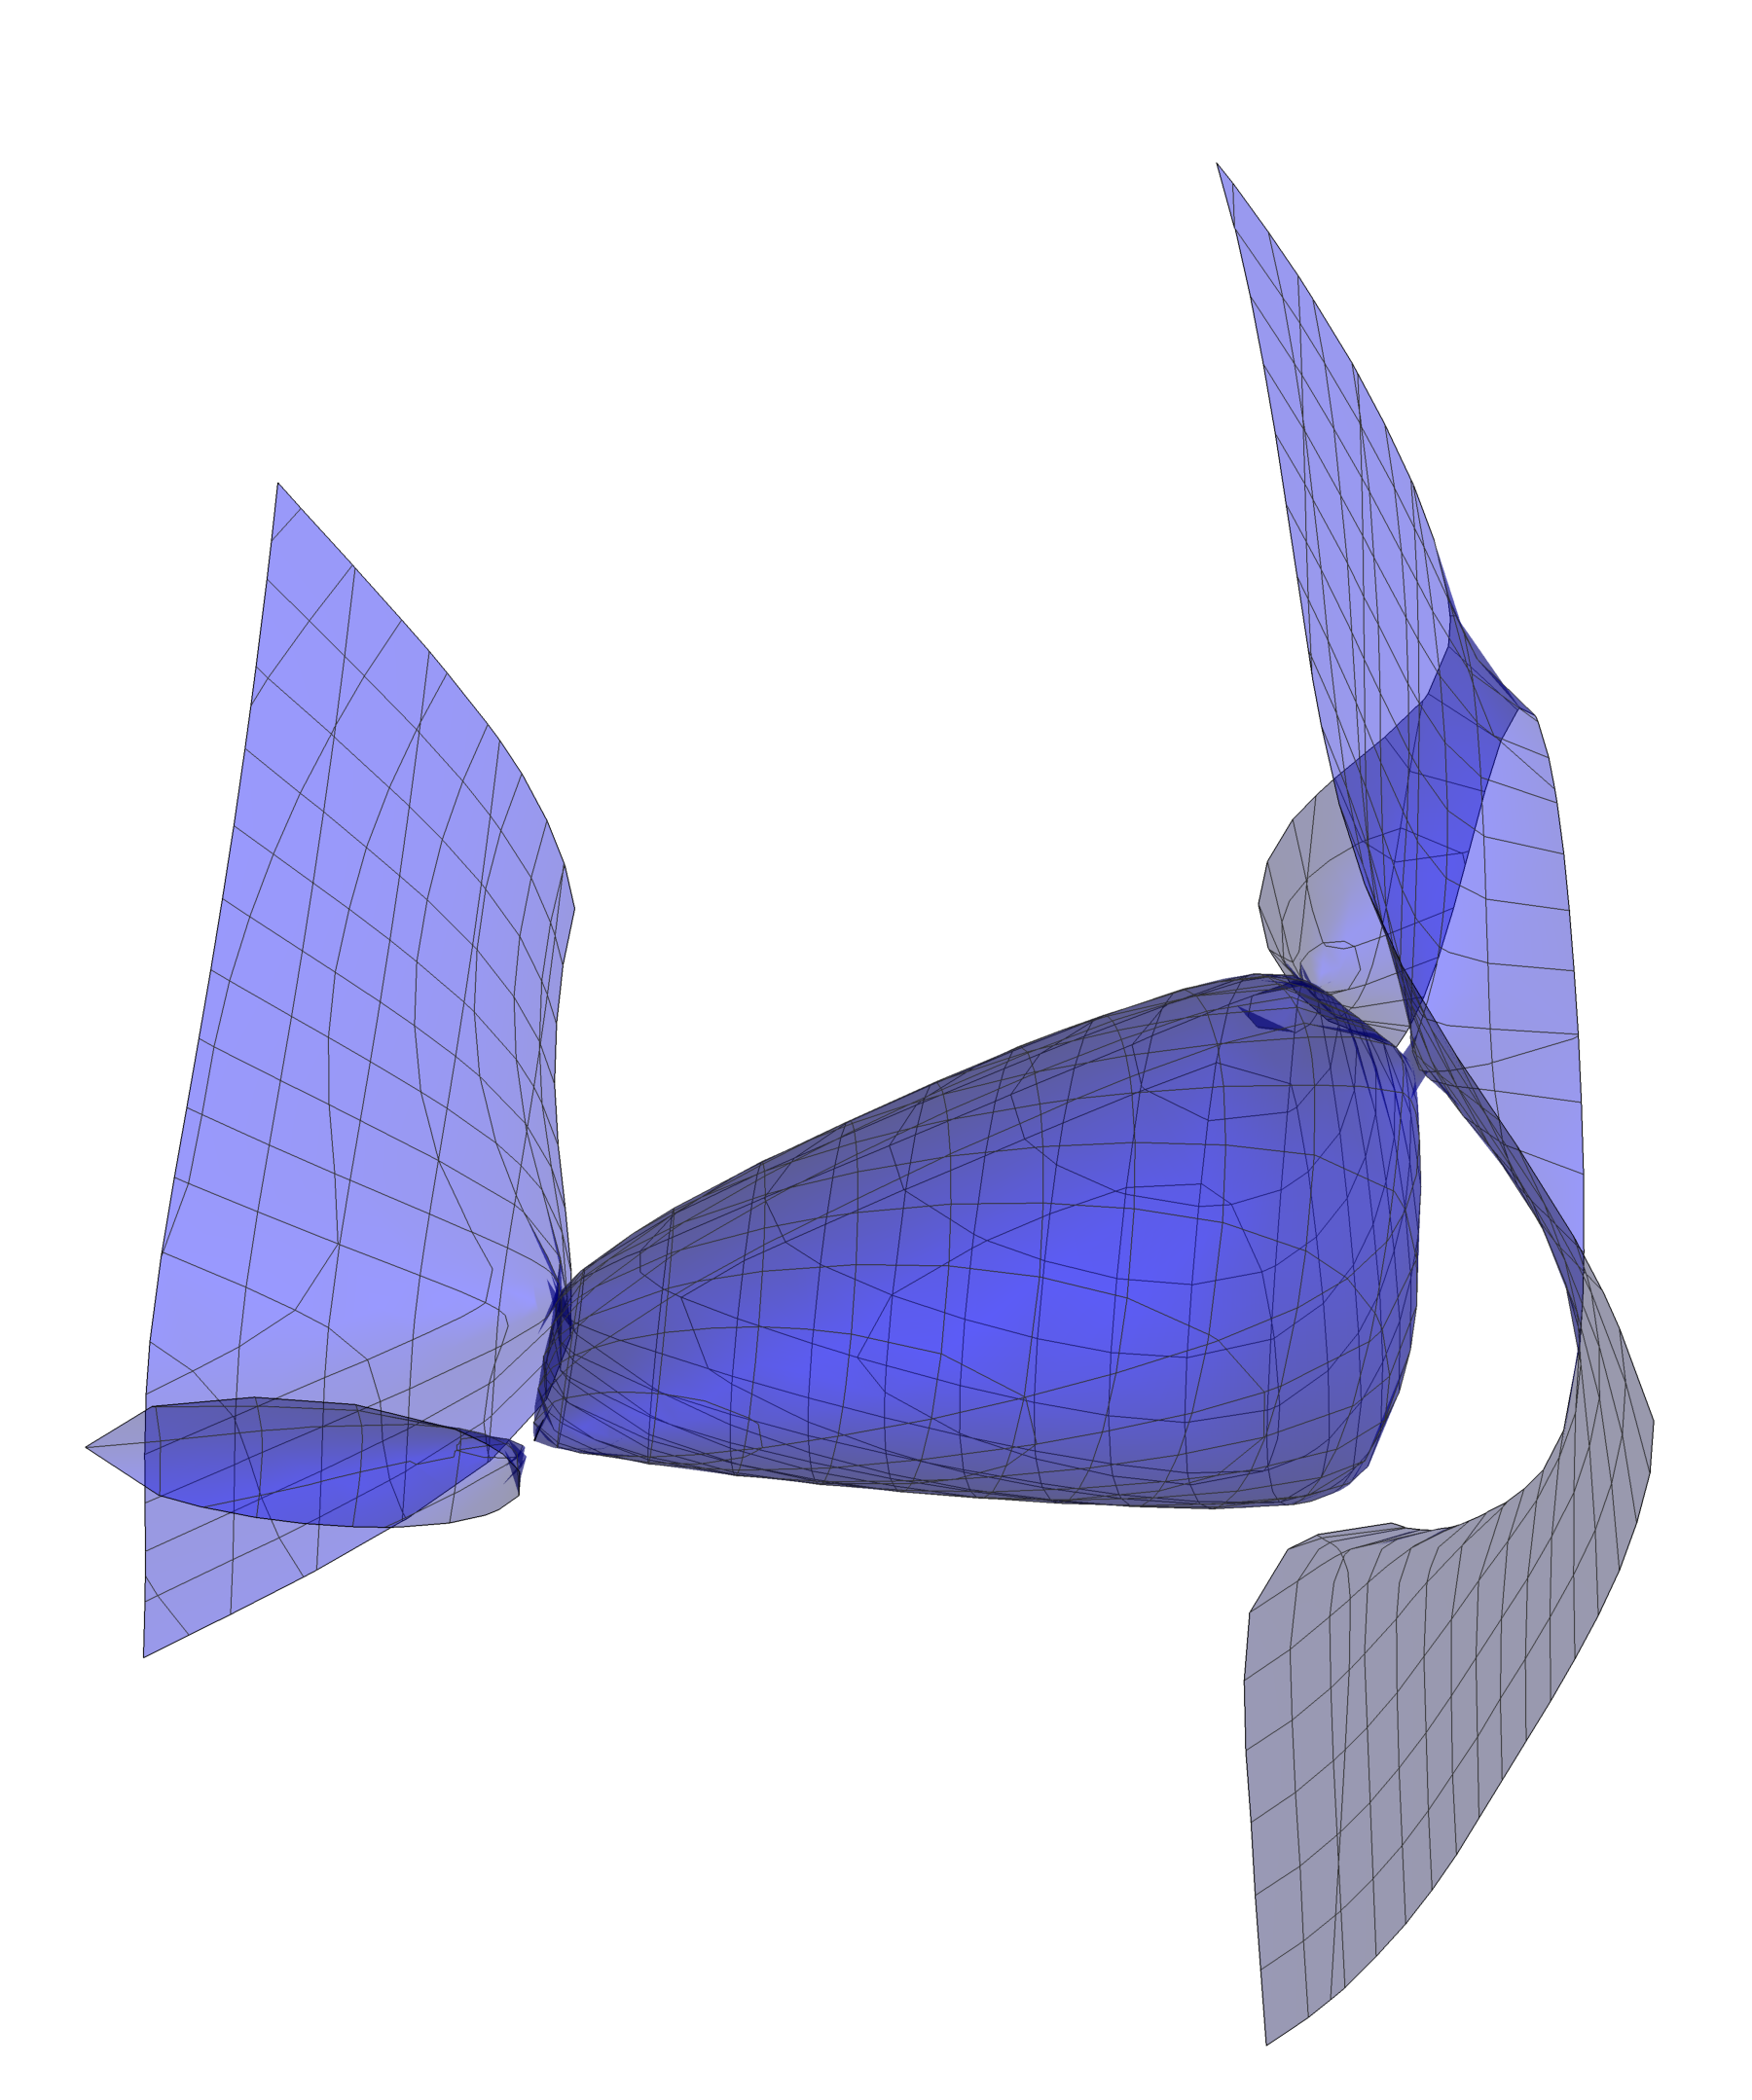
\includegraphics[width=.3\linewidth]{IMAGES/Hyp_Deriv_g}
    \hspace{0.5cm}
    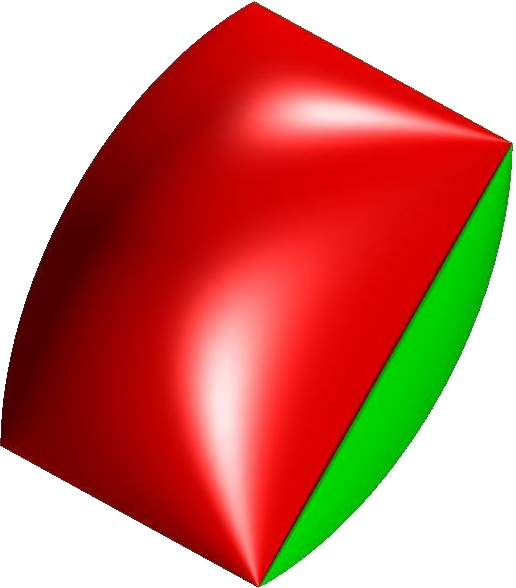
\includegraphics[width=.25\linewidth]{IMAGES/honest_pillow}
    \hspace{0.5cm}
    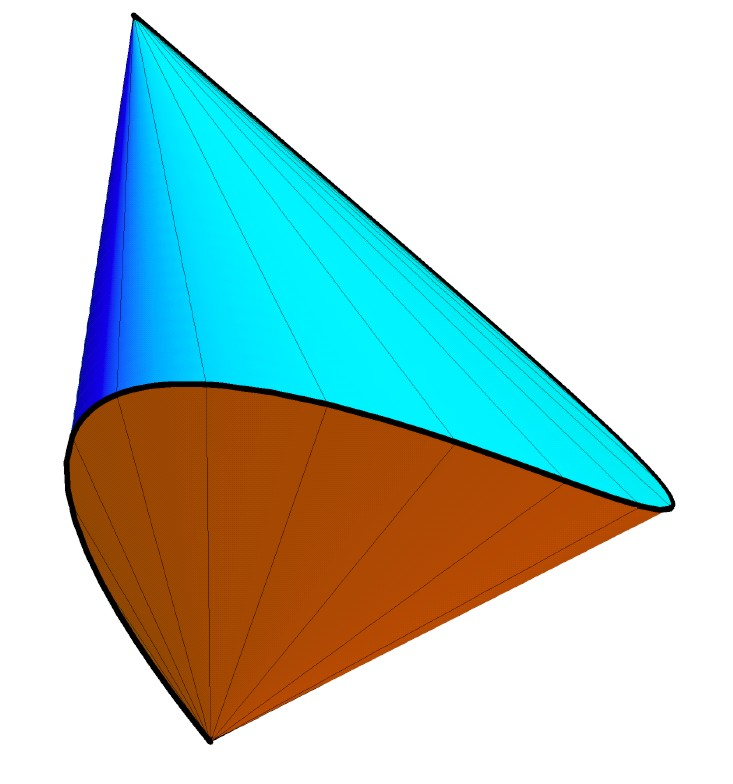
\includegraphics[width=.25\linewidth]{IMAGES/T4}
  \end{figure}
\end{frame}


%%%%%%%%%%%%%%%%%%%%%%%%%%%%%%%%%%%%%%%%%%%%%%%%%%%%%%%%%%%%%%%%%%%%%%%%%%%%%
\begin{frame}
\frametitle{\vspace{-0.5cm}\bc \bf Motivations and properties\ec}

\vspace{-0.5cm}
\begin{itemize}
\item[] Polyhedra $\rightarrow$ feasible sets of {\color{blue} Linear Programming} ({\color{blue} LP})
  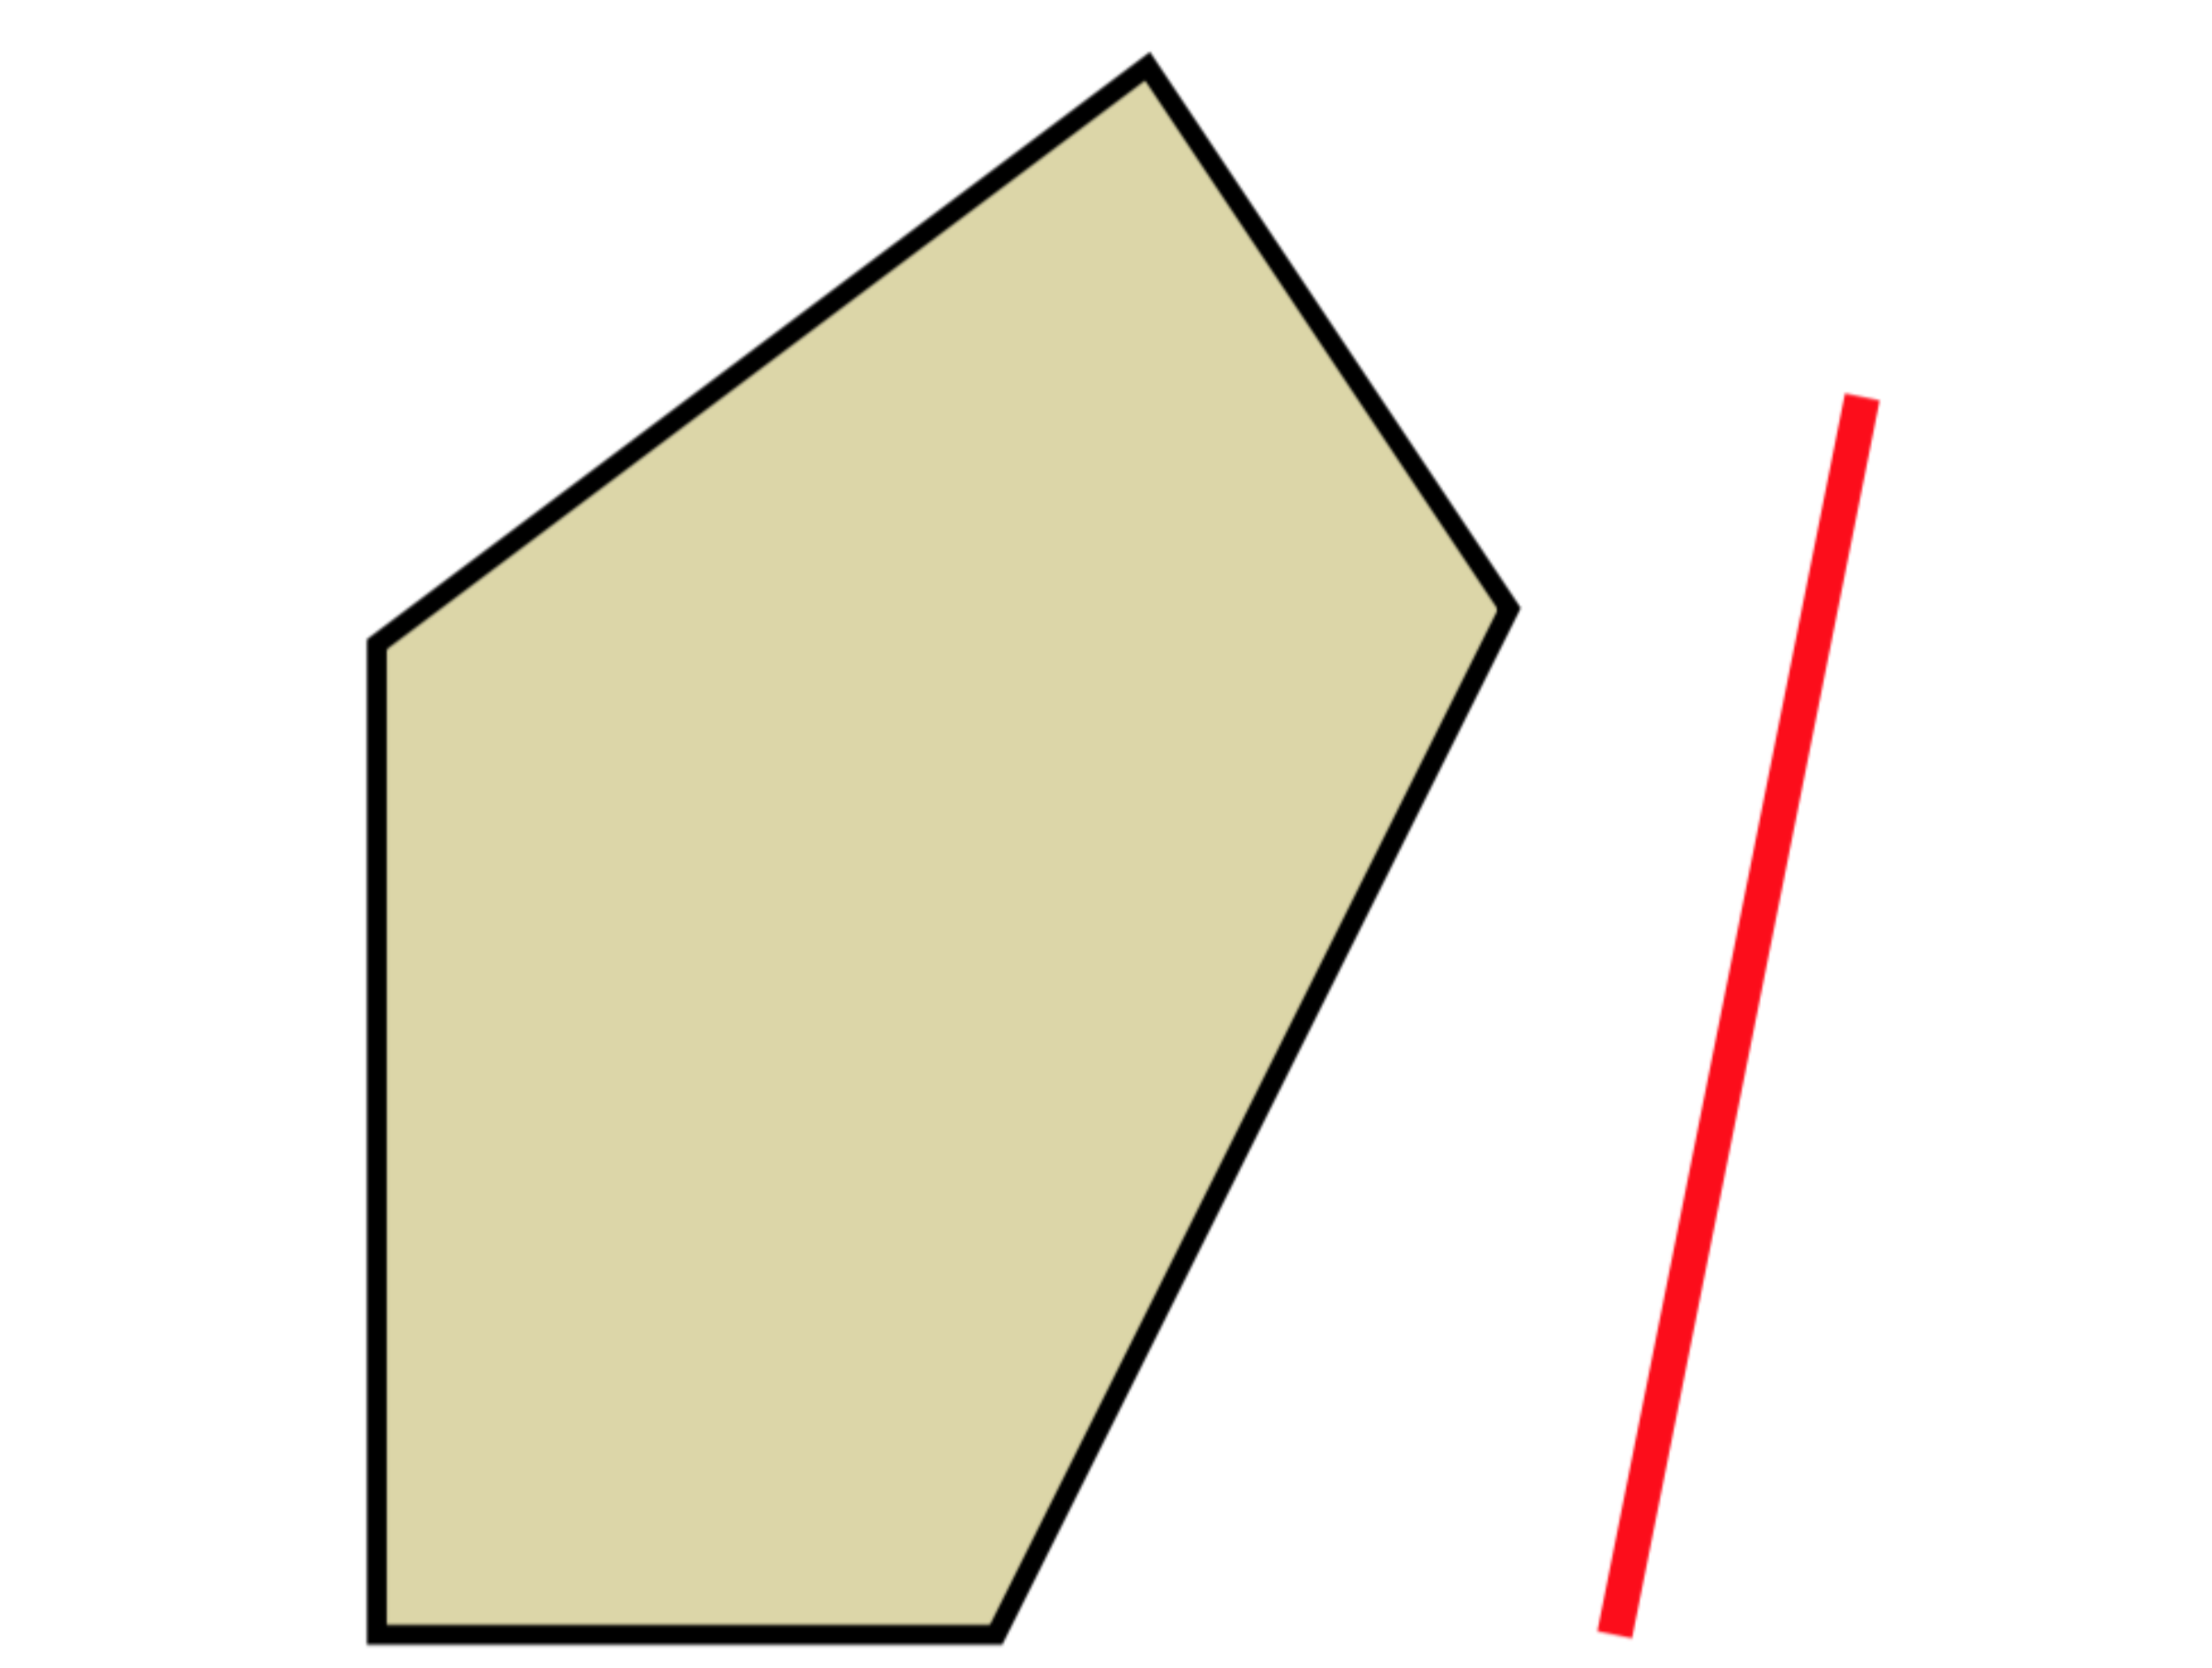
\includegraphics[scale=0.025]{IMAGES/LP_types}
  \vspace{-0.4cm}
\item[] Spectrahedra $\rightarrow$ feasible sets of  {\color{blue} Semidefinite Programming} ({\color{blue} SDP})
  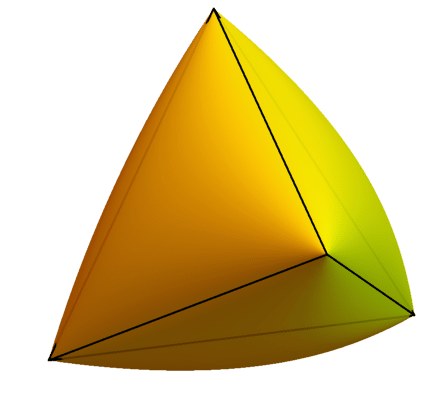
\includegraphics[scale=0.06]{IMAGES/cayley_yellow}
\end{itemize}
\vspace{0.2cm}

\pause

Classical applications from
\begin{itemize}
\item
  {\color{blue} real algebraic geometry} (positive polynomials vs SOS, 17th Hilbert's problem)
\item
  {\color{blue} control theory} (Lyapunov stability)
\item
  {\color{blue} combinatorial optimization} (e.g. SDP relaxation of MAXCUT)
\item
  {\color{blue} polynomial optimization} (moment-SOS relaxation hierarchy)
\end{itemize}

\pause
\vspace{0.2cm}

Several {\bf \color{blue} common properties} besides convex/semialgebraic, for instance:

\begin{itemize}
\item closed under intersection
\item exposed faces, ...
\end{itemize}

\vspace{0.2cm}
\pause

but spectrahedra/SDP are highly more {\bf \color{red} pathological} than polyhedra/LP:

\begin{itemize}
\item spectrahedra are {\only<5->{\color{olive}\bf}not closed under linear image}
\item solutions only over algebraic extension:
  \scalebox{0.8}{
    $\{\sqrt{2}\} = \left\{x \in \RR :
    \left[\begin{smallmatrix} x & 1 \\ 2 & x\end{smallmatrix}\right] \succeq 0
    \text{ and }
    \left[\begin{smallmatrix} 1 & x \\ x & 2\end{smallmatrix}\right] \succeq 0\right\}$
    }
  %  (points of spectrahedra might not be representable over the defining field)
\item
  in SDP: weak infeasibility, not attainement of inf/sup, etc...
\end{itemize}

\end{frame}


%%%%%%%%%%%%%%%%%%%%%%%%%%%%%%%%%%%%%%%%%%%%%%%%%%%%%%%%%%%%%%%%%%%%%%%%%%%%%
\begin{frame}
\frametitle{\vspace{-0.5cm}\bc \bf Semidefinite representable sets\ec}

The linear projection of a spectrahedron is called a {\color{blue} spectrahedral shadow}:
$$
S = \left\{x \in \RR^n : \exists\, y \in \RR^p, A_0 + \sum_{i=1}^n x_i A_i + \sum_{j=1}^p y_j B_j \succeq 0\right\},
$$
for matrices $A_i,B_j \in \sym^d$. \pause
Spectrahedra and their shadows are in general called {\color{blue} semidefinite representable sets}.
\pause

\begin{figure}
  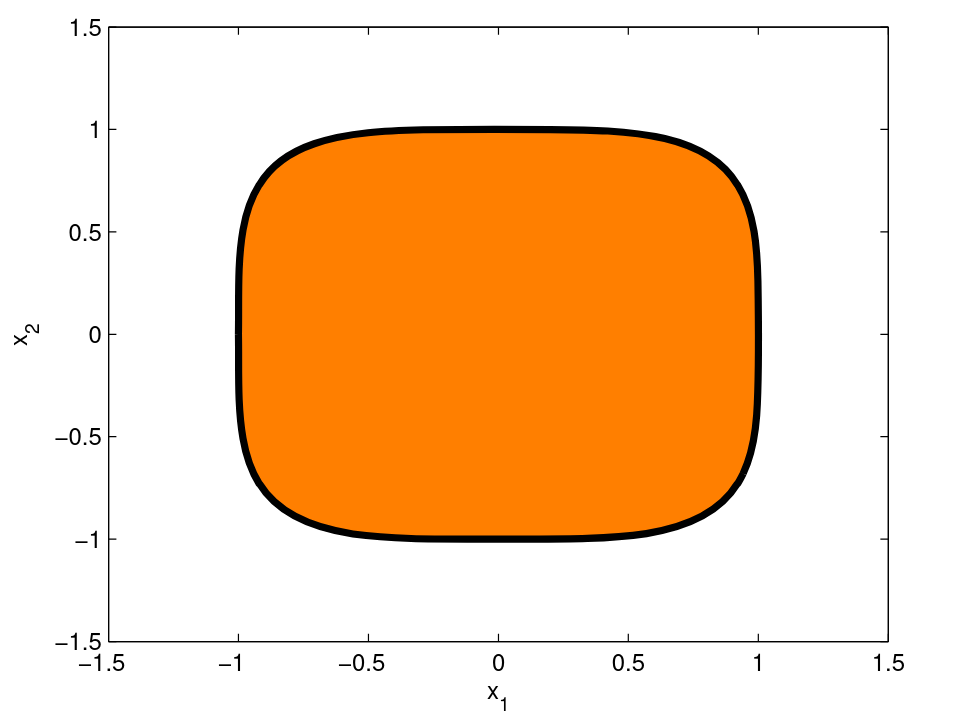
\includegraphics[scale=0.1]{IMAGES/fermat4}
  \centering
  \caption*{\hfill The convex hull of the Fermat's quartic $x^4+y^4=1$ \\
    \hfill is semidefinite representable but not spectrahedral}
\end{figure}
\pause

Not every convex (compact) semialgebraic set is semidefinite representable (Scheiderer, 2018).

\end{frame}

%Given $C,M_1,\ldots,M_n \in \SS_m(\RR)$ and $b \in \RR^k$:
%  \begin{columns}[t,onlytextwidth]
%    \begin{column}{0.4\textwidth}
%      \bc{\bf Primal SDP}\ec
%      \begin{align*}
%        p^* = \inf_{X \in \mathbb{S}_m} & \,\,\, (C,X):=Trace(CX) \\
%         s.t.         & \,\,\, {\color{red} X \succeq 0} \\
%        & {\color{red} (M_j,X)=b_j, j=1, \ldots, k}
%      \end{align*}
%    \end{column}
%    \begin{column}{0.6\textwidth}
%      \bc{\bf Dual SDP}\ec
%      \begin{align*}
%        d^* = \sup_{s \in \RR^k} & \,\,\, b's \\
%        s.t.       & \,\,\, {\color{red} M(s) \succeq 0} \\
%         & {\color{red} M(s)=C-s_1M_1-\cdots-s_kM_k} 
%      \end{align*}
%    \end{column}
%  \end{columns}
%\pause




%%%%%%%%%%%%%%%%%%%%%%%%%%%%%%%%%%%%%%%%%%%%%%%%%%%%%%%%%%%%%%%%%%%%%%%%%%%%%
%\begin{frame}
%\frametitle{\vspace{-0.5cm}\bc \bf \Huge Positivity certificates of polynomials \ec}
%Say I want to certify that
%\[
%f=U_1^4+U_1U_2^3+U_2^4-3U_1^2U_2U_3-4U_1U_2^2U_3+2U_1^2U_3^2+U_1U_3^3+U_2U_3^3+U_3^4
%\]
%is globally nonnegative ($f(u) \geq 0$ for all $u \in \RR^3$). \,\,\,\, 
%%\pause
%{\it E.g.}, is it a {\color{orange} \bf Sum Of Squares}?
%%\pause
%\vspace{0.2cm}
%\bc Does there exist a PSD Gram matrix for $f$? \ec
%\vspace{0.2cm}
%
%\begin{tcolorbox}[colback=green!5,colframe=gray!40!black]
%\setbeamercolor{mybox}{bg=orange}
%\begin{beamercolorbox}[sep=1mm]{mybox}
%$\text{With } \langle v \rangle_\RR = \RR[U]_2 \,\,\,\,\,\,\,\,\,\,\, \mathscr{S} = \{X \in \SS^6(\RR) \mymid f=v'Xv, X \succeq 0\} \neq \emptyset\,?$
%\end{beamercolorbox}
%\end{tcolorbox}
%\vspace{0.4cm}
%%\pause
%\red{Bad news\,/\,Interesting facts} about this example:
%\begin{itemize}
%\item $f \in \sum (\RR[U]_2)^2$ but $f\notin\sum (\QQ[U]_2)^2$
%\item Hence $\mathscr{S}$ is degenerate and $\mathscr{S} \cap \SS^6(\QQ) = \emptyset$
%\item $f$ is never a sum of 3 non-zero squares (but it is of $2$)
%\end{itemize}
%\end{frame}




%%%%%%%%%%%%%%%%%%%%%%%%%%%%%%%%%%%%%%%%%%%%%%%%%%%%%%%%%%%%%%%%%%%%%%%%%%%%%
%\begin{frame}
%\frametitle{\vspace{-0.5cm}\bc \bf \Huge Multivariate polynomial optimization \ec}
%
%\begin{tcolorbox}[colback=green!50,colframe=blue!30!black,title=\bc {\bf The general problem} \ec]
%  \bc $f^*=\displaystyle\inf_{x \in {\color{red} \bf S}} f(x)$, \,\,\, with \,\,\,{\color{red} ${\color{red} \bf S} = \{x \in %\RR^n \mymid {\bf g_1}(x) \geq 0, \ldots, {\bf g_s}(x) \geq 0\}$} \ec
%\end{tcolorbox}
%
%\begin{itemize}
%\item[$\bullet$] If ${\color{red} \bf S}=\RR^n \longrightarrow f^*=\displaystyle\sup_{\lambda \in \RR} \lambda$ \,\,
%  s.t. \,\, $f(x)-\lambda \geq 0 \,\,\,\,\forall\,\,x\in \RR^n$ \,\, {\bf [NP-hard]}
%\item[] Write $f-\lambda$ as a sum of squares? $f-\lambda= f_1^2+\cdots+f_p^2$ \,\,\, {\bf \color{blue} [SDP]}
%\item[] Hilbert (1888): Positivity $\equiv$ SOS iff ${\color{olive} n=1}$ or ${\color{olive} d=2}$ or ${\color{olive} (n,d)=(2,4)}$
%\pause
%\vspace{0.2cm}
%\item[$\bullet$] When ${\color{red} \bf S}$ is any set : {\bf Positivestellensatz}
%\bc  (Schm\"udgen) \,\,${\color{red} \bf S}$ \,compact\,\,:\,\,
%$f-y = \displaystyle\sum_{\nu \in \{0,1\}^s}\sigma_{\nu}\prod_j{\bf \color{red} g_j}^{\nu_j}$ \,\, with $\sigma_i$ SOS  \,\, {%\bf \color{blue} [SDP]} \ec
%\bc  (Putinar) \, \,\,\,\,${\color{red} \bf S}$ archimedean\,\,:\,\,\,
%$f-y = \sigma_0 + \displaystyle\sum_i\sigma_i{\bf \color{red} g_i}$ \,\,\,\,\,\,\, with $\sigma_i$ SOS  \,\, {\bf \color{blue} [SDP]} \ec
%\pause
%\vspace{0.2cm}
%\item[$\bullet$] Lasserre ('01), Parrilo ('03) \ldots Moments vs SOS approach also gives {\bf \color{blue} [SDP]}
%\end{itemize}
%
%\end{frame}


%%%%%%%%%%%%%%%%%%%%%%%%%%%%%%%%%%%%%%%%%%%%%%%%%%%%%%%%%%%%%%%%%%%%%%%%%%%%%
%\begin{frame}
%\frametitle{\vspace{-0.5cm}\bc \bf \Huge State of the art \ec}
%
%\vspace{-0.3cm}
%
%\setbeamercolor{mybox}{bg=gray}
%\begin{beamercolorbox}[sep=1mm]{mybox}
%${\bf Fixed\hspace{-0.1cm}-\hspace{-0.1cm}Precision \,\, Polynomial\hspace{-0.1cm}-\hspace{-0.1cm}Time \,\, Algorithms\,\, for\,\, SDP}$
%\end{beamercolorbox}
%{\cit Shor, Nemirovsky, Yudin ('60s-'70s), \ldots, }{\cit Khachiyan}\\
%Ellipsoid algorithm is $Poly(m,n,\log(1/\epsilon))$ : {\color{red} inefficient in practice} \\
%{\cit Nesterov, Nemirovsky ('90s)}\\
%Interior point algorithms : {\color{blue} efficient in practice}
%
%{\cit Ramana, Khachiyan, Porkolab ('90s)}\\
%Complexity bounds for LMI : {\color{blue} can't be used in practice}
%
%\pause
%
%\vspace{0.1cm}
%
%\setbeamercolor{mybox}{bg=gray}
%\begin{beamercolorbox}[sep=1mm]{mybox}
%${\bf (Rational)\,points\,in\,(convex)\,Semialgebraic\,Sets}$
%\end{beamercolorbox}
%{\cit Peyrl, Parrilo (2007), Kaltofen, Li, Yang, Zhi (2008)}\\
%Floating-point-SOS $\rightarrow$ Rational approximation $\rightarrow$ Projection on the feasible set \\
%{\cit Guo, Safey El Din, Zhi (2013)} \\
%Bit complexity bounds for emptiness of $\{x \in \QQ^n \mymid \red{A}(x) \succeq 0\}$\\
%
%\pause
%
%\vspace{0.1cm}
%
%\setbeamercolor{mybox}{bg=gray}
%\begin{beamercolorbox}[sep=1mm]{mybox}
%${\bf Exact\,\,algorithms\,\,for\,\,LMI/SDP}$
%\end{beamercolorbox}
%{\cit Henrion, N., Safey El Din (2015-2016)} \\
%New upper bounds for emptiness of $\{x \in \RR^n \mymid \red{A}(x) \succeq 0\}$ \\
%{\cit N. (2016)} \\
%Rank-constrained SDP \hfill (poly-time if \, $n$ \, {\bf or} \, $m=\text{size}({A})$ \, is fixed)
%
%%Open questions:
%%\begin{itemize}
%%\item
%%How if $\{x \in \QQ^n \mymid \red{A}(x) \succeq 0\}=\emptyset$?
%%\item
%%Additional rank constraints?
%%\end{itemize}

%\end{frame}




\end{document}
